\section{Overføringsfunktionen for Buck-konverterens udgangsfilter}\label{sec:spm1}
\begin{figure}[h!]
	\centering
	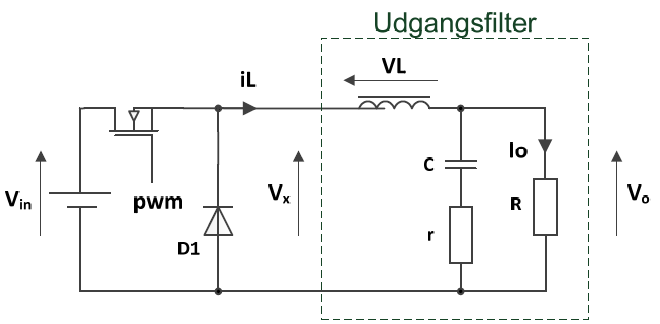
\includegraphics[width=.8\textwidth]{udgangsfilter.png}
	\caption{Buck-konverterens udgangsfilter indrammet af den stiplede linje.}
	\label{fig:udgangsfilter}
\end{figure}
\FloatBlock

Overførelsesfunktion $G(s) = \frac{v_o(s)}{V_x(s)}$ for Buck-konverterens udgangsfilter som ses i fig (\ref{fig:udgangsfilter})\footnote{Kilde : Regulering, Aktivitet 1, Modellering af en Buck-konverters udgangsfilter. 3/10-2016 KHA}

\begin{align}
V_o(s) &= V_x(s) \cdot \left( \frac{\left(\frac{1}{sC} + r \right) || R }{sL + \left(\frac{1}{sC} + r \right) || R}  \right) 
\quad, \quad hvor \frac{1}{SC} + r || R = \frac{R+sCrR}{1+sCr+sCR} \\
\Rightarrow G(s) &= \frac{v_o(s)}{V_x(s)} = \frac{ \frac{R+sCrR}{1+sCr+sCR}}{sL +  \frac{R+sCrR}{1+sCr+sCR}} \\
&= \frac{R+sCrR}{sL+s^2CLr+s^2CLR+R+sCrR}\\
&= \frac{1+sCr}{\frac{sL}{R}+\frac{s^2CLr}{R}+s^2CL+sCr}\\
&= \frac{1}{LC} + \frac{sCr+1}{s^2\left(\frac{r}{R}+1\right)+s\left(\frac{1}{RC}+\frac{r}{L}\right)+\frac{1}{LC}} \label{eq:transferfunction_g}
\end{align}
Som det ses i ligning (\ref{eq:transferfunction_g}), er der tale om et 2. ordens lavpass filter.